\chapter{Desenvolvimento}

Esta seção tem por propósito apresentar o estudo realizado sobre a
\textit{startup} Rua Dois Tecnologias, sendo esta o objeto de análise
central do presente trabalho. O escopo deste capítulo abrangerá desde
o entendimento sobre o contexto da empresa e sua proposta de valor
até aspectos mais técnicos como a arquitetura do sistema atual e
problemas que já são enfrentados pela \textit{startup} nessa arquitetura.

  As seções estão dispostas em:

  \begin{description}
    \item[Rua Dois Tecnologias:] breve apresentação sobre a empresa e os
      serviços que esta oferece.
    \item[Arquitetura do sistema:] descrição da arquitetura de software atual
      adotada dentro da Rua Dois, e possíveis soluções discutidas dentro da
      empresa a respeito da escalabilidade.
  \end{description}

\section{Rua Dois Tecnologias}

No artigo \textit{Modernizing Real Estate: The Property Tech Opportunity}
\footnote{\url{https://www.forbes.com/sites/valleyvoices/2019/02/22/the-proptech-opportunity}},
a autora \citeonline{LouisaXu} aborda uma visão histórica sobre o desenvolvimento
de tecnologias para o mercado imobiliário fazendo um comparativo com a realidade atual.
Nesse histórico de desenvolvimento, ela relata que desde 1980 são empregados
diversos esforços na área buscando melhorarias por meio de software, mas mesmo
assim, continuamos em uma ramo altamente burocrático e carente de melhorias.

Ciente dessas limitações, PAULO SOBRENOME fundou em outubro de 2018 a
Rua Dois Tecnologias, com o propósito de solucionar as dificuldades
enfrentadas tanto por parte das imobiliárias quanto por parte dos locatários
\footnote{Aquele que mora em um imóvel que não lhe pertence, mediante um
contrato de locação.} no processo de locação de imóveis.

CONVERSAR COM O ERLAN PARA MELHORAR ESSA PARTE

% TODO Conversar com o Erlan para melhorar essa parte
% TODO Explicar o que é CEO e colocar nas lista de abreviações
% TODO Verificar com a Fernanda se tudo bem incluir o nome dela no TCC
% TODO Descrever melhor o contexto e os papeis envolvidos

\subsection{Serviços prestados}

Visando o processo de locação de imóveis, a Rua Dois conta com quatro serviços
sendo desenvolvidos dentro da empresa, afim de agregar valor aos seus clientes,
sendo eles:

  \begin{enumerate}
    \item \textbf{Captação de Imóveis:} serviço destinado à atrair proprietários de
      imóveis que desejam divulgar o imóvel para locação.
    \item \textbf{Visitas:} serviço de visitas aos imóveis, no qual os interessados em
      locar o imóvel agendam um horário para conhecer o mesmo.
    \item \textbf{Propostas:} serviço no qual os interessados, após passarem pela etapa
      de visitação, avaliam o imóvel e fazem uma proposta para o proprietário do
      imóvel referente ao valor a ser pago pela locação e possíveis ajustes que
      desejam que sejam feitos na propriedade.
    \item \textbf{Contrato:} etapa final, destinada a automatizar a avaliação por parte
      das seguradoras, envio de documentos e assinatura do contrato.
  \end{enumerate}

Cada serviço é vendido de forma separada para as imobiliárias, de forma que cada uma
adapte ao seu contexto os serviços que melhor se encaixam. Atualmente, o serviço
mais desenvolvido é o de visitas e a equipe vem trabalhando com o intuito de
estabilizar os demais serviços.

\section{Arquitetura do sistema}

\subsection{Arquitetura atual}

A arquitetura atual do sistema é composta por dois sistemas principais -
\textit{r2service} e \textit{r2visit}, responsáveis por gerir a maior parte
das funcionalidades relacionadas aos serviços de visitas, propostas, e contrato -
e uma série de sistemas auxiliares e outros serviços que auxiliam no ciclo de
vida do produto. A Figura \ref{fig:ArquiteturaAtual} visa ilustrar esse sistema,
o qual será descrito a seguir:

\begin{figure}[h]
  \centering
  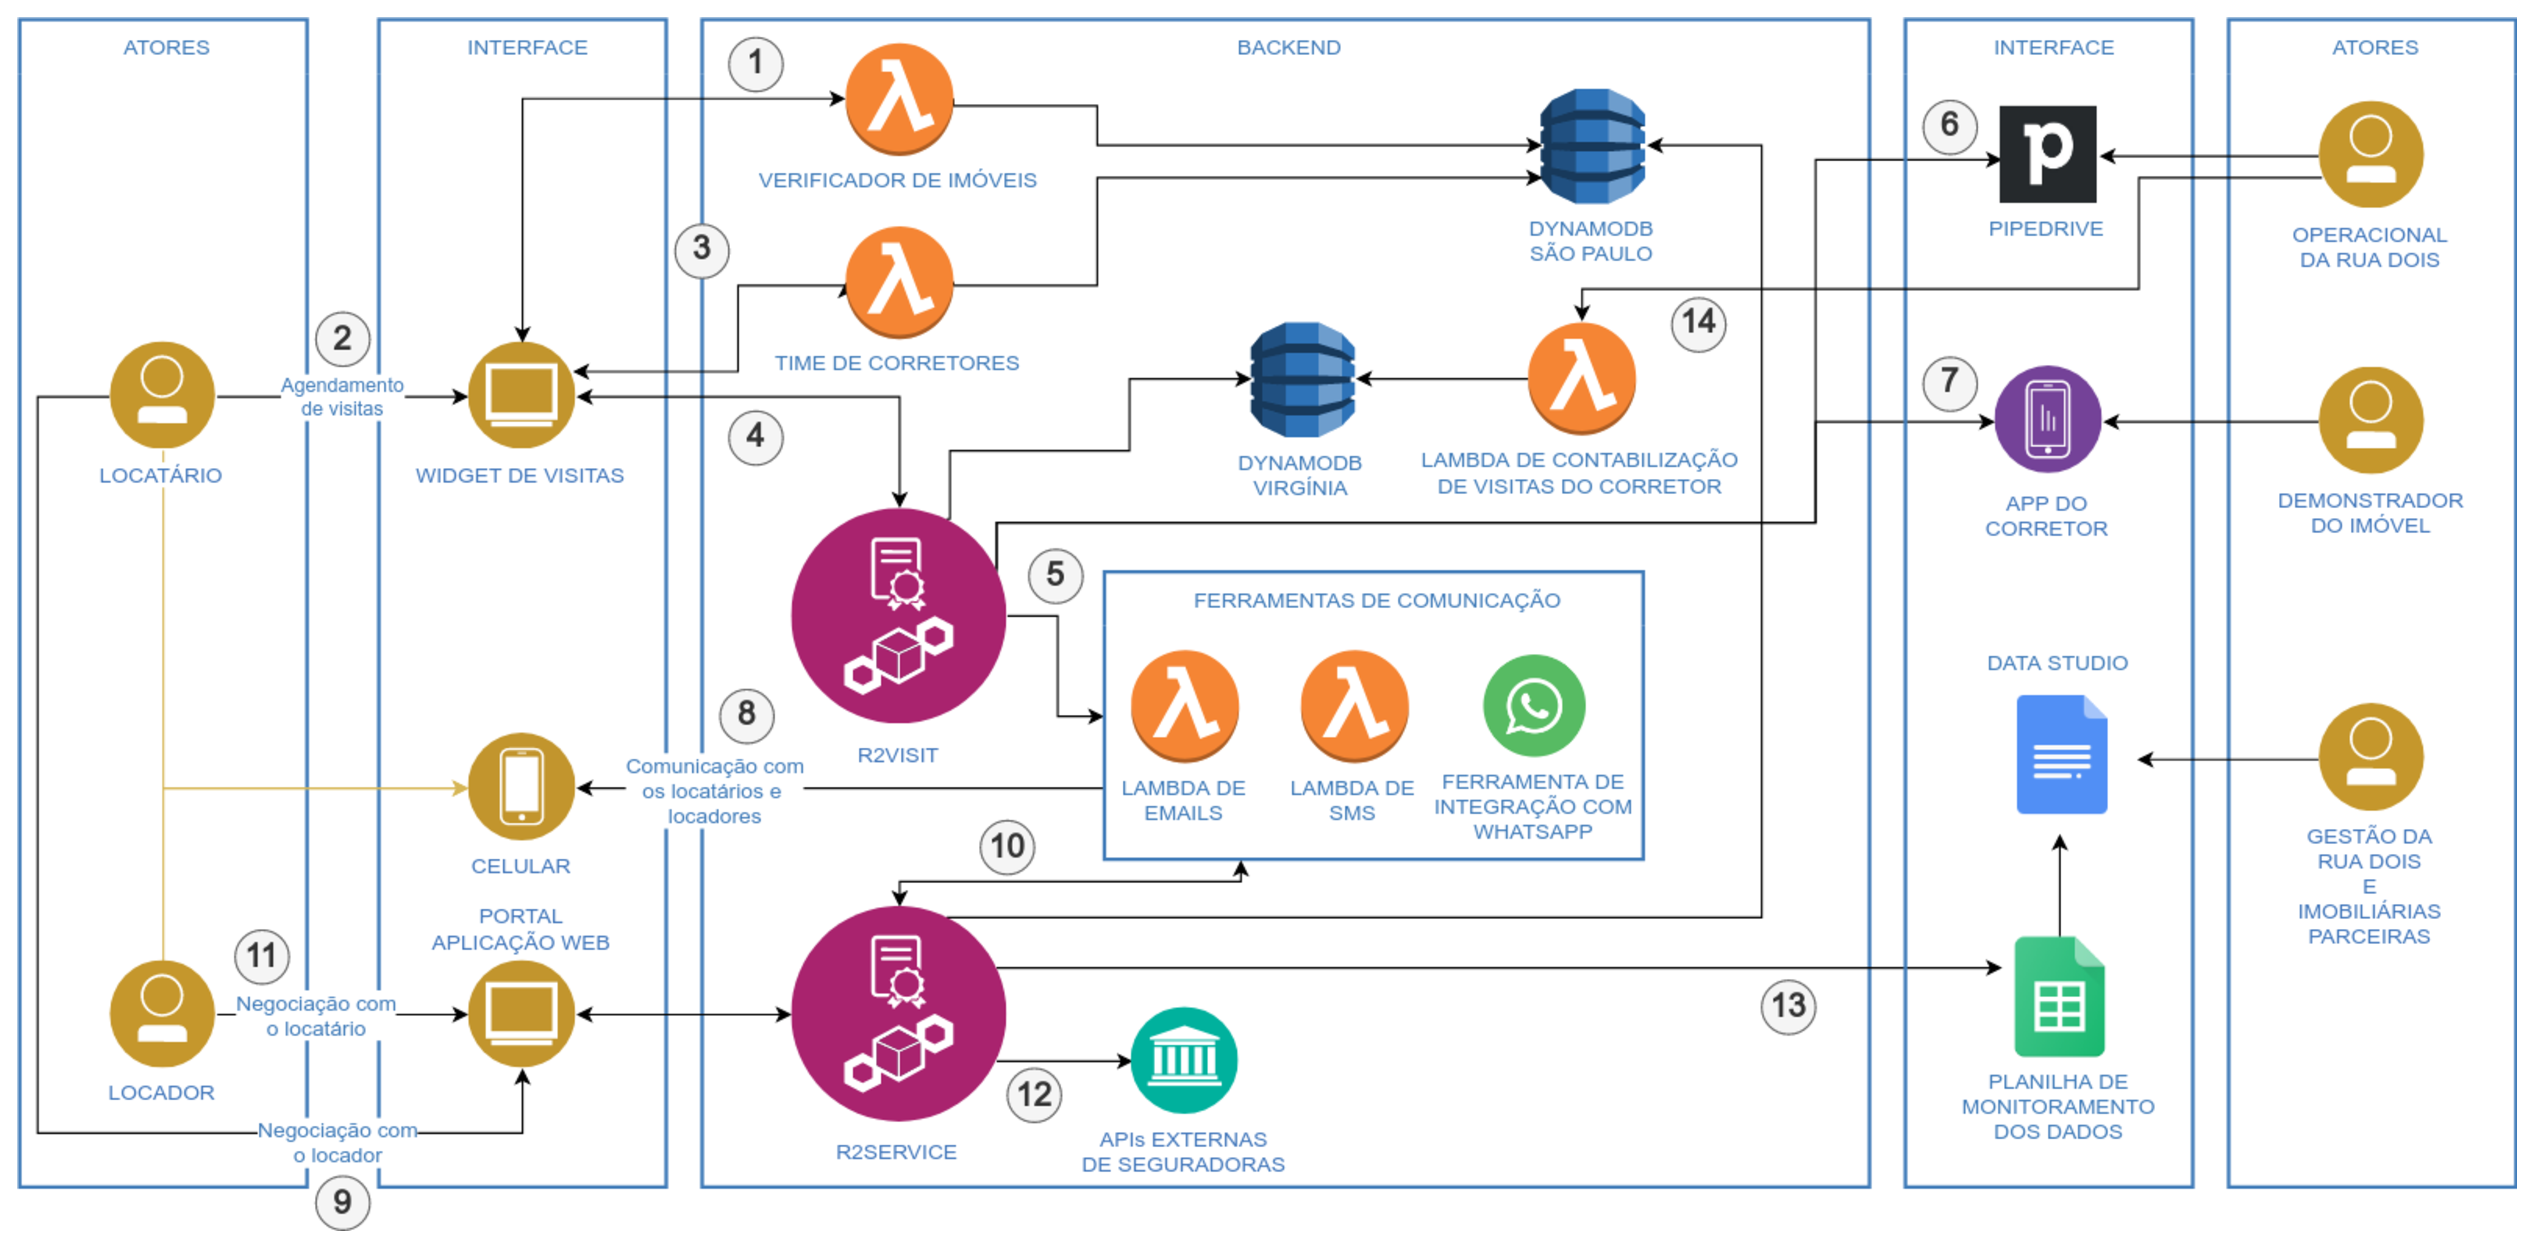
\includegraphics[keepaspectratio=true,scale=0.3]{figuras/r2ArquiteturaAtual.eps}
  \caption{Arquitetura atual do sistema da Rua Dois}
  \label{fig:ArquiteturaAtual}
\end{figure}

  \begin{enumerate}
    \item O \textit{Widget} é um componente utilizado pela Rua Dois que roda
      no \textit{frontend} dos sites das imobiliárias que aderem ao serviço
      de visitas. Ele se comunica com um lambda responsável por verificar se
      o imóvel apresentado no site da imobiliária está disponível no banco
      de dados da Rua Dois. Uma vez que esteja disponível, o \textit{widget}
      exibe um botão que disponibiliza o agendamento da visita \textit{online}
      para o interessado.
    \item O locatário ao clicar nesse botão, dispara uma requisição ao lambda
    que identifica o time de corretores responsável por atender as visitas
    ao imóvel selecionado. E em seguida, uma nova requisição é disparada ao
    serviço \textit{r2visit} solicitando o calendário com os horários
    disponíveis do respectivo time.
    \item Após o locatário ter selecionado o horário da visita, uma nova
    requisição é lançada para registrar a visita no \textit{r2visit}, que por
    sua vez dispara uma série de mensagens por meio das ferramentas de comunicação
    e atualiza o Pipedrive\footnote{O Pipedrive é uma ferramenta de CRM -
    \textit{Customer Relationship Management} utilizada pela empresa para
    realizar o gerenciamento operacional e monitoramento dos resultados obtidos.
    Saiba mais em: \url{https://www.pipedrive.com}}.
    \item Após a visita ser realizada, o corretor sinaliza por meio do aplicativo
    a conclusão da visita, disparando novamente no \textit{r2visit} os eventos
    de atualização do Pipedrive e as ferramentas de comunicação, para que se
    possa dar início a nova fase de Negociação, referente ao produto de propostas.
    \item Nessa nova fase, locatário e locador trocam mensagens por meio do portal
    da Rua Dois, o qual é gerido pelo \textit{r2service}. Ao final da negociação,
    os cliente entram na fase de contrato, na qual seus dados são recolhidos e
    enviados por meio do \textit{r2service} para APIs externas de seguradoras as quais
    realizam uma avaliação de crédito do locatário. Quando concedida a avaliação
    de crédito, o contrato é gerado automaticamente com os dados já recolhidos
    do locatário, locador, da imobiliária e do próprio imóvel.
    \item Por fim, o \textit{r2service} é responsável por atualizar uma planilha do
    Google Sheets\footnote{Saiba mais em: \url{https://www.google.com/sheets/about/}}
    que serve de insumo para geração de relatórios dentro do Data Studio
    \footnote{Saiba mais em: \url{https://datastudio.google.com}}.
  \end{enumerate}

\subsection{Problemas enfrentados}

Desde seu início, a Rua Dois tem em seu modelo de negócio uma constante
preocupação com a escalabilidade do sistema. A empresa tem em seus objetivos
validar rapidamente a ideia e expandir para diferentes mercados. Contudo,
este objetivo foi alinhado a uma equipe de desenvolvimento de software
inexperiente tanto no contexto de desenvolver software para \textit{startups}
quanto em questões de qualidade e arquitetura de software. A soma desses
dois fatores gerou uma série de decisões equivocadas sobre a arquitetura
desse sistema que hoje atrapalham sua evolução ao invés de facilitar o
crescimento escalável da empresa. Dentre estas decisões estão:

  \begin{enumerate}
    \item A escolha de usar um banco não-relacional - DynamoDB - em um
    contexto extremamente relacional. Atualmente existem seis entidades
    principais dentro do sistema: imobiliária, imóvel, cliente, corretor,
    visita e proposta. Todas dispostas em tabelas diferentes do DynamoDB,
    o que implica que todos os relacionamentos entre as entidades são
    construídos a nível de aplicação. A documentação do DynamoDB diz:
      \begin{quotation}
        "Em geral, você deve manter o mínimo de tabelas possível em um
        aplicativo do DynamoDB. A maioria dos aplicativos bem-projetados exige
        somente uma tabela." \cite{doc:dynamodbModeling}.
      \end{quotation}
    A Rua Dois foi contrária a essa recomendação, e trabalha com uma tabela
    para cada entidade. De forma que, toda a eficiência que eles
    buscavam em fazer consultas com um banco de dados NoSQL, é perdida
    no mal planejamento do projeto em cima desse arquitetura.
    \item A adoção de microsserviços sem conhecer a real demanda dos
    serviços que seriam oferecidos. Sendo uma \textit{startup}, a Rua Dois
    se caracteriza por um ambiente extremante incerto, de validação de ideias.
    Oleksiy Kovyrin, chefe do Swiftype\footnote{\url{https://swiftype.com/}},
    disse em entrevista a \citeonline{JakeLumetta}:
      \begin{quotation}
        "Toda vez que consideramos a introdução de um novo serviço, temos que
        considerar o custo operacional de fazer isso. Cada novo serviço aumenta a
        complexidade da infraestrutura e torna um pouco mais difícil raciocinar
        sobre as relações de serviço dentro do sistema."
      \end{quotation}
    Dado o contexto da Rua Dois, no qual não se tem domínio sobre o produto final
    que será entregue somado a uma equipe sem experiência de trabalho com microsserviços,
    a escolha mais segura seria um sistema monolítico \cite{JakeLumetta}.
    Atualmente, a empresa enfrenta dificuldades de manter essa arquitetura,
    compartilhar o conhecimento sobre a mesma com novos integrantes e, principalmente,
    manter a consistência dos dados. Esse último é o fator de maior impacto
    na arquitetura, uma vez que se tem diversos microsserviços compartilhando
    o uso das mesmas tabelas, além de tabelas duplicadas em serviços diferentes,
    nas quais é necessário estar realizando constantemente a sincronização dos dados.

    \item Optar por usar a infraestrutura na Amazon Web Services, a qual
    possui diversos recursos mas também possui maior complexidade para
    configurá-los do que outras ferramentas disponíveis no mercado \cite{kavya}.
    Completando o quadro de utilizar uma arquitetura de microsserviços, com
    uma equipe inexperiente, a empresa ainda enfrenta as dificuldades de manter
    essa arquitetura que não é trivial, em uma infraestrutura que também exige
    determinados conhecimentos que atualmente o time de desenvolvimento
    não possui.
  \end{enumerate}


  % Não é preciso o widget solicitar o time, o r2visit deve ser capaz de fazer isso pelo imóvel


